\chapter{Conclusions}
\label{ch:conclusions}

\textbf{This chapter is now complete - but wasn't in the first three chapter draft submission!}

In conclusion, this project assesses Rust as suitable for performant and production implementations of High-Performance Computing codebases, answering the titular question. This conclusion is as a result of three factors.

Firstly, \Cref{ch:translation} shows that it is possible to translate non-trivial existing codebases representative of High-Performance Computing workloads from C++ into Rust, including leveraging both shared and distributed memory parallelism through the \texttt{rayon} and \texttt{mpi} crates. It further shows that these translations provide significant benefits to developer productivity. These include reduced effort spent debugging as a result of memory and concurrency safety guarantees and the rich type system, along with quantitative models of productivity using the \texttt{scc} tool suggesting only $0.61 \times$ the total cost is required to complete develop a codebase with equivalent functionality leveraging both shared and distributed memory parallelism in Rust.

Secondly, \Cref{ch:performance} shows that the performance of Rust translations of non-trivial C++ codebases closely approaches their reference implementations, with at worst around a $1.5 \times$ slow-down incurred across parallelism strategies. This measured slow-down concurs with existing literature, such as Moran and Bull's ``Emerging Technologies: Rust in HPC'' \cite{moranEmergingTechnologiesRust2023}, and is likely because the dominant kernel in HPCCG, sparse matrix-vector multiplication, is less amenable to compiler optimisation in Rust than in C++. Since this kernel is very common in High-Performance Computing, this impacts its suitability for these workloads. However, other literature such as Constanzo et al. \cite{costanzoPerformanceVsProgramming2021} examining less High-Performance Computing specific kernels such as the N-body problem find that Rust is equally performant in these cases. In addition to this, the Rust translations exhibit similar strong and weak scaling properties to the original C++ implementations, demonstrating its capability to scale to the extent required for High-Performance Computing workloads.

These first two factors can be interpreted together by plotting a graph comparing the empirical performance and estimated productivity of the C++ and Rust implementations of the HPCCG mini-app, as shown in Figure \ref{fig:conclusions_performance_productivity}. This figure visualises the result that C++ offers fair performance gains over Rust, but development of Rust programs is likely to improve development productivity.

\begin{figure}[H]
    \centering
    % This file was created with tikzplotlib v0.10.1.
\begin{tikzpicture}

\definecolor{darkorange25512714}{RGB}{255,127,14}
\definecolor{darkslategray38}{RGB}{38,38,38}
\definecolor{lightgray204}{RGB}{204,204,204}
\definecolor{steelblue31119180}{RGB}{31,119,180}

\begin{axis}[
axis line style={lightgray204},
height=0.45\textheight,
legend cell align={left},
legend style={fill opacity=0.8, draw opacity=1, text opacity=1, draw=none},
tick align=outside,
tick pos=left,
title={Performance vs. Productivity in C++ and Rust for HPC},
width=\textwidth,
x grid style={lightgray204},
xlabel=\textcolor{darkslategray38}{Estimated cost of development [\$]},
xmajorgrids,
xmin=10161.2, xmax=47182.8,
xtick style={color=darkslategray38},
y grid style={lightgray204},
ylabel=\textcolor{darkslategray38}{Total runtime for 200x200x200 mesh [s]},
ymajorgrids,
ymin=6.4475, ymax=71.4025,
ytick style={color=darkslategray38}
]
\path [draw=black, semithick]
(axis cs:11844,57.5)
--(axis cs:11844,58.7);

\path [draw=black, semithick]
(axis cs:11980,11.73)
--(axis cs:11980,11.81);

\path [draw=black, semithick]
(axis cs:27553,58.23)
--(axis cs:27553,58.33);

\path [draw=black, semithick]
(axis cs:27723,68.07)
--(axis cs:27723,68.45);

\path [draw=black, semithick]
(axis cs:31665,43)
--(axis cs:31665,44.2);

\path [draw=black, semithick]
(axis cs:31970,9.4)
--(axis cs:31970,10.2);

\path [draw=black, semithick]
(axis cs:45180,48.63)
--(axis cs:45180,48.73);

\path [draw=black, semithick]
(axis cs:45500,35.7)
--(axis cs:45500,36.04);

\addplot [semithick, black, mark=x, mark size=3, mark options={solid,draw=steelblue31119180}, only marks]
table {%
11844 58.0999984741211
11980 11.7700004577637
27553 58.2799987792969
27723 68.2600021362305
};
\addlegendentry{C++}
\addplot [semithick, black, mark=x, mark size=3, mark options={solid,draw=darkorange25512714}, only marks]
table {%
31665 43.5999984741211
31970 9.80000019073486
45180 48.6800003051758
45500 35.8699989318848
};
\addlegendentry{Rust}

\draw (axis cs:11944,58.1) node[
  scale=0.4165,
  anchor=base west,
  text=black,
  rotate=0.0
]{serial};
\draw (axis cs:12080,11.77) node[
  scale=0.4165,
  anchor=base west,
  text=black,
  rotate=0.0
]{rayon};
\draw (axis cs:27653,58.28) node[
  scale=0.4165,
  anchor=base west,
  text=black,
  rotate=0.0
]{mpi};
\draw (axis cs:27823,68.26) node[
  scale=0.4165,
  anchor=base west,
  text=black,
  rotate=0.0
]{hybrid};
\draw (axis cs:31765,43.6) node[
  scale=0.4165,
  anchor=base west,
  text=black,
  rotate=0.0
]{serial};
\draw (axis cs:32070,9.8) node[
  scale=0.4165,
  anchor=base west,
  text=black,
  rotate=0.0
]{openmp};
\draw (axis cs:45280,48.68) node[
  scale=0.4165,
  anchor=base west,
  text=black,
  rotate=0.0
]{mpi};
\draw (axis cs:45600,35.87) node[
  scale=0.4165,
  anchor=base west,
  text=black,
  rotate=0.0
]{hybrid};

\end{axis}
\end{tikzpicture}

    % 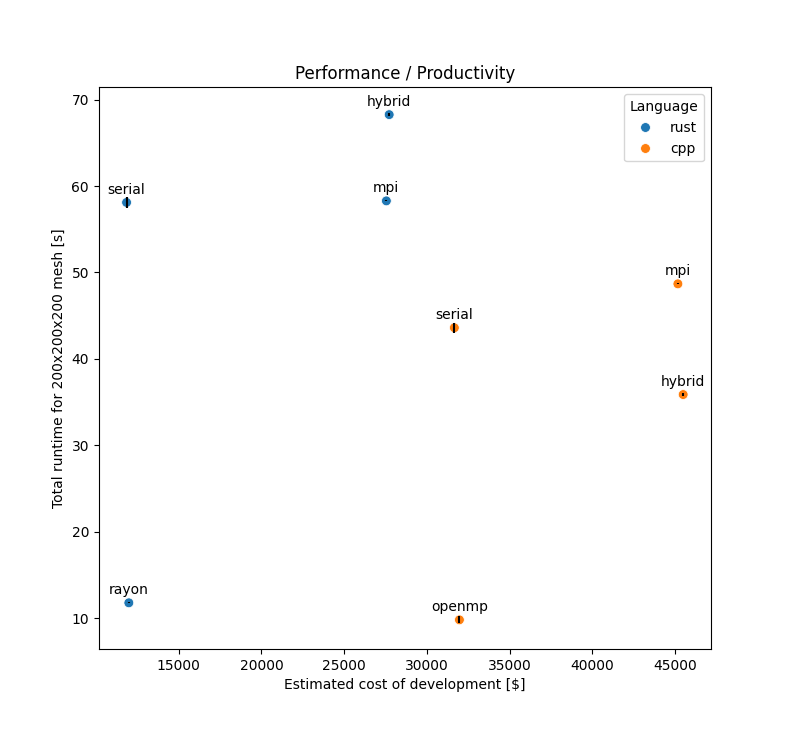
\includegraphics[width=\textwidth]{images/7_conclusions/performance_productivity.png}
    \caption{A comparison of performance and productivity between the C++ and Rust languages.}
    \label{fig:conclusions_performance_productivity}
\end{figure}

% TODO: Check up on hybrid re-runs
% scc . --exclude-file Cargo.lock --exclude-dir target
% scc . --exclude-file .gitignore YAML* dump_matlab*

The final factor which impacts the conclusion is that the performance and productivity of Rust is likely to improve faster than for C++. This is because it is a relatively young language, whose package ecosystem and optimising compilers are yet to reach maturity. As a result of this, there is likely more scope for improvement and less technical debt than with C++, facilitating a faster rate of improvement.

These factors taken in combination demonstrate Rust's suitability for High-Performance Computing applications, as despite its performance not matching C++ for the measured computational kernels, it provides commensurate benefits in developer productivity such as its compiler guarantees of memory and thread safety.
% , which might make it preferable for real-world applications bounded by budget.


\section{Future work}
\label{sec:future-work}

% TODO: Make this not first person?
Firstly, I am aiming to submit a paper derived from this project to the P3HPC (Performance, Portability and Productivity in High-Performance Computing) 2024 workshop, as a result of the three novel contributions discussed in \Cref{ch:introduction}.
% TODO: Re-iterate these contributions

In addition to this, whilst HPCCG is around an order of magnitude longer than any of the Rust codebases examined in existing literature, it is one of the shortest mini-apps in the Mantevo suite. In addition to this, although HPCCG is ``the original Mantevo mini-app'', other mini-apps in the suite are more influential and commonly used. As a result of this, one avenue for future work is translating and analysing a longer, more influential mini-app, for example MiniMD \cite{osti_1231191} or HPCG \cite{dongarra2015hpcg}.

Finally, equivalence checking is a very broad and complex field. As such, future work could easily be derived from this section. For example, a framework implementing the proof-of-concept approach leveraging \texttt{autocxx} as part of a translation methodology could be developed. For example, a crate using Rust macros for ergonomic multiplexing between C++ and Rust function calls could be created for this purpose. In addition to this, comparison of generated LLVM IR for equivalence checking was dropped as out of scope for this project, but could still yield fruitful research.

% In addition to this, publicising and maintaining open source tools requires a lot of effort from developers. To maximise the impact of the HPC MultiBench, a final possible avenue of future work is making it easily accessible, including publishing it on to the Python Package Repository, and responding to bug and feature requests raised on GitHub.


\section{Reflection}
\label{sec:reflection}

% TODO: Re-work this paragraph
On reflection, I am immensely proud of the work I have completed in the course of this project. Coming in to the project, I did not have a good way to estimate how long translation tasks, so generously scheduled time in my project specification to undertake these tasks. It transpired that I was able to complete the translation of the serial and parallel implementations faster than expected, which allowed me to focus on the stretch goals of the project. The initially planned stretch goal was extending the translation effort to include an assessment of the Rust bindings to MPI. This presented an interesting technical challenge of using complex Rust structures within an API which does not exactly map to the C++ implementation of the MPI specification.

% This project was a success, as it achieved all of its ``Must have'' and ``Should have'' objectives, shown in Appendix \ref{sec:project-requirements}. These include translating, equivalence checking, and undertaking a performance analysis of a High-Performance Computing mini-app across serial, shared memory, and distributed memory parallelism approaches. In addition to this, two ``Could have'' objectives relating to the equivalence checking were dropped, which allowed time for the development of tooling for reproducibly running and aggregating performance experiments. This tool facilitated deep performance analysis of the HPCCG translation, but also stands on its own as a helpful utility for engineers working in High-Performance Computing, as validated by the industry review.

In addition to this, empowered by incredibly helpful conversations with my supervisor, I also chose to extend the project by building tooling to facilitate performance measurements on High-Performance Computing resources using Slurm. I found this very fulfilling, as I personally enjoy building tooling which can improve difficult processes in the real world. In my opinion, this is one of the stand-out aspects of this project, as it not only was it incredibly helpful during my performance analysis, but can also be used as an open source software product going forward.

Finally, I believe that this project extends existing literature on the topic to a meaningful degree with three novel contributions. Firstly, it provides a translation and assessment of suitability for an application which is both around an order of magnitude longer than the largest existing work, and more representative of common High-Performance Computing workloads. This assessment is also broader in scope than those in existing literature, including distributed memory parallelism with MPI, and leveraging sophisticated techniques such as roofline models and strong and weak scaling analyses. Secondly, it proposes both a novel approach and novel tool to mitigate issues within translation and reproducible performance analysis, making future work in the field easier to undertake.


\section{Open source work}
\label{sec:open-source-work}

The open source community is critical in publishing and maintaining much of the infrastructure powering the modern world. In the course of this project, I developed a number of open source contributions.

Due to the departmental regulations on open source contributions, the vast majority of open source contributions developed during this project are currently embargoed in private repositories, which will then be made public after the assessment phase of the project has completed. However, there are some exceptions to this rule, which were made with supervisor approval.

\section{Contributions already released}
\label{ssec:open-source-already-released}

Firstly, when developing the novel equivalence checking approach leveraging foreign-function interfaces in Rust with \texttt{autocxx}, I needed to invoke functions using array parameters. There was an open issue (\url{https://github.com/google/autocxx/issues/989}) on the project stating that some support for arrays had recently been added, but that this functionality was untested. To resolve this, I pull requested integration tests for this functionality (\url{https://github.com/google/autocxx/issues/989}, shown in Appendix \ref{sec:autocxx-pull-request-appendix}), which confirms its correctness and prevent regression in future.

This pull request has since been merged into the main branch of this repository, and as such will be included in the next release of the \texttt{autocxx} tool. Since this functionality is very common in High-Performance Applications, this confirmation of support unblocks applying this technique in future work

Secondly, during the initial mini-app identification phase of the project, I noticed that some of the links on the UK-MAC website were broken. As a result of this, I raised a GitHub issue for this (\url{https://github.com/UK-MAC/uk-mac.github.com/issues/1}), and then made a pull request to fix these links (\url{https://github.com/UK-MAC/uk-mac.github.com/pull/2}). This pull request has since been merged, and the website now works correctly.

Finally, I made a pull request into the HPCCG repository to add Doxygen-style docstrings to the mini-app, based on the understanding that I gained during the translation process (\url{https://github.com/Mantevo/HPCCG/pull/5}). However, since this project was last actively developed seven years ago, this pull request has not been reviewed nor merged.

\section{Contributions to be released}
\label{ssec:open-source-to-be-released}

Firstly, the HPC MultiBench tool repository will be made public, and published on PyPI so it can be installed using the \texttt{pip} package manager. In addition to this, the generated run data and test plan YAML files for the performance analysis of HPCCG and the replication trial of Moran and Bull's paper \cite{moranEmergingTechnologiesRust2023} will be included as example submodules in the release.

Secondly, all code from the Rust translation effort will be made public. In addition to this, corollary work from this effort, such as the modernisation of HPCCG's build system to use CMake and unit tests using the Catch2 framework, will be pull requested into the HPCCG repository. Finally, the Kokkos version of HPCCG will also be made public, and a link to it pull requested into \url{https://github.com/kokkos/kokkos-miniapps}, a repository containing a list of mini-apps with Kokkos translations.

% \begin{enumerate}
%     \item Make public the HPC MultiBench tool, and publish it on PyPI so it can be installed using the \texttt{pip} package manager
%     \item Make public the Rust translation of the HPCCG mini-app
%     \item Make public the run results generated using the HPC MultiBench tool for the Rust translation of HPCCG and the replication trial of Moran and Bull's paper \cite{moranEmergingTechnologiesRust2023}
%     \item Pull request modernisation of the build system for the HPCCG mini-app to use CMake
%     \item Pull request unit tests using the Catch2 framework written the for HPCCG mini-app
%     \item Pull request a link to Kokkos version of the HPCCG mini-app into \url{https://github.com/kokkos/kokkos-miniapps}, a repository containing a list of mini-apps with Kokkos translations
% \end{enumerate}

% Finally, I intend to write then make the following contributions once the project has been assessed:

% \begin{enumerate}
%     \item Pull request documentation for using arrays as function arguments in \texttt{autocxx}, following up on the pull request discussed in the previous section \url{https://github.com/google/autocxx/pull/1353#issuecomment-1961615591}
%     \item Pull request documentation including and annotating integration tests as examples for the \texttt{mpi} crate, following up on issue \url{https://github.com/rsmpi/rsmpi/issues/174#issuecomment-1961638459}.
% \end{enumerate}
